\documentclass[11pt]{article}
\usepackage{../stat110}
\usepackage{graphicx}
\usepackage{epigraph}
\usepackage{hyperref}

%\STAFF

\begin{document}
\SectionNotes{7}{Normals, Uniforms, etc}{Luis Perez (luisperez@college.harvard.edu)}{Aidi Zhang (aidizhang@college.harvard.edu)}

\setlength{\epigraphwidth}{.6\textwidth}
\epigraph{“But to us, probability is the very guide to life.”}{Joseph Butler}

\section*{Practice Problems}
\begin{exercise}[Secret Santa]
For Christmas, $n$ people are doing a Secret Santa, where each person puts his or her name on a piece of paper in a hat and randomly picks a name from the hat without replacement. In this game, there is a possibility that people can select their own names and have to buy themselves a gift. :(
 \begin{enumerate}[a)] \itemsep 1.5in
         \item What is the expected number of cycles that form? What is the expected number as $n \rightarrow \infty$? The secret santa chain depicted on the right would have 3 cycles.\\

         \begin{center}
         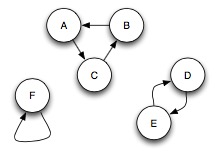
\includegraphics[scale=0.6]{cycles.jpg}
         \end{center}

         \item What is the approximate distribution of the number of people who draw their own names if $n$ is large? What is $P(X=0)$ under this approximation?

 \end{enumerate}
\end{exercise}

\begin{solution}
\begin{enumerate}
\item
Let $X$ be the number of cycles that form. We break down $X$ into indicator variables $X = I_1 + I_2 + ... + I_n$ where $I_j$ is the indicator for whether the $j$th person in Secret Santa completes a cycle after drawing a name from the hat.\\

We apply linearity of expected value adn the fundamental bridge to express the expected value of $X$ in terms of the probabilities of each of the 100 events.

$$E(X) = P(I_1 = 1) + P(I_2 = 1) + ... + P(I_n = 1)$$

We note that $P(I_1 = 1) = 1/n$ for the first person to choose, the only way that that person will from a cycle is for him to choose himself. This pattern continues until $P(I_n = 1) = 1$ as the last person who draws will always complete a cycle. Thus we have that

$$E(X) = \frac{1}{n} +\frac{1}{n-1} + ...+\frac{1}{1} = \sum_{k=1}^n \frac{1}{k}$$

This is the harmonic series, which diverges as $n \rightarrow \infty$.

\item For large $n$, $X$ is approximately $Pois(1)$. As a result as $n \rightarrow \infty$, $P(X = 0) \rightarrow \frac{1}{e}$.
\end{enumerate}
\end{solution}

\pagebreak

\begin{exercise}
Courtesy of Jessy Hwang) Let $U_{2, 3} \sim \Unif(2,3)$ and let $Z \sim \N(0,1)$, where $U_{2, 3}$ is independent of $Z$.
 \begin{enumerate}[a)] \itemsep 1.5in
         \item Using $U_{2, 3}$, construct a r.v. $X$ whose CDF is $F(x) = 1 - \displaystyle\frac{1}{(1+x)^4}$ for $x \ge 0$.
         \item Write down an integral for $E(X)$, where $X$ is the r.v. from part $a$. You do not need to evaluate this integral.
         \item Find $P(U_{2, 3} \ge 2.5, Z > 2 | Z > 0)$ in terms of the standard Normal CDF $\Phi$, and approximate this probability.
         \item Find $E(U_{2, 3}^2)$.
         \item Describe how one could produce a sample observed value for $Z$ given a sample observed value of $U_{0, 1}$.
\end{enumerate}
\end{exercise}

\begin{solution}
\begin{enumerate}
\item We have that $U_{2,3} - 2 \sim Unif(0,1)$. By Universality of Uniform, $U_{2,3} - 2 \sim F(X)$, so $X \sim F^{-1}(U_{2,3} - 2)$. Therefore, we have that $X = (3 - U_{2,3}^{-1/4}) - 1$ has the desired CDF.

\item By LOTUS, based off our answer in part a, we have that

$$E(X) = \int_{2}^{3} ((3-u)^{-1/4} - 1)du$$

\item We have that

\begin{align*}
P(U \ge 2.5, Z > 2 | Z > 0) &= P(U \ge 2.5|Z>2, Z>0)P(Z>2|Z>0) \\
&= P(U_{2,3} \ge 2.5)P(Z>2|Z>0) \\
&= \frac{1}{2}2(1-\Phi(2)) = 1 - \Phi(2)
\end{align*}

\item By symmetry,

$$E(U_{2,3}^2) = E((U_{0,1} + 2)^2)$$

We multiply out and apply linearity,

$$E((2 + U_{0,1})^2) = E(U_{0,1}^2 + 4U_{0,1} + 4) = E(U_{0,1}^2) + 4E(U_{0,1}) + 4$$

We know that $E(U_{0,1}) = \frac{1}{2}$ and we can find $E(U_{0,1}^2)$ knowing the variance of $U$ and applying one of the definitions of variance.

\begin{align*}
Var(U_{0,1}) &= E(U_{0,1}^2) - E(U_{0,1})^2 \Rightarrow \frac{1}{12} = E(U_{0,1}^2) + (\frac{1}{2})^2 \\
E(U_{0,1}^2) &= \frac{1}{3}
\end{align*}

Then,

$$E((2+U_{0,1})^2) = E(U_{0,1}^2) + 4E(U_{0,1}) + 4 = \frac{1}{3} + 4(\frac{1}{2}) + 4 = \frac{19}{3}$$

\item By Universality of Uniform, $U_{0,1} \sim \Phi(Z)$, where $\Phi$ is the CDF of a standard normal distribution. As a result, given a random draw of $U_{0,1}$, we have that $Z \sim \Phi^{-1}(U_{0,1})$ adn so $\Phi^{-1}(U_{0,1})$ would yield a sample observed value for $Z$.

\end{enumerate}
\end{solution}

\pagebreak

\begin{exercise}[The Pareto distribution]
The Pareto distribution with parameter $a > 0$ has PDF $f(x) = \frac{a}{x^{a+1}}$ for $x \ge 1$ (and 0 otherwise). This distribution is often used in statistical modeling.

\begin{enumerate}
\item Find the CDF of a Pareto distribution with parameter $a$; check that it is a valid CDF.

\item Suppose that for a simulation you want to run, you need to generate i.i.d. Pareto(a) r.v.s. You have a computer that knows how to generate i.i.d. Unif(0,1) r.v.s but does not know how to generate Pareto r.v.s. Show how to do this.
\end{enumerate}
\end{exercise}

\begin{solution}
Homework problem :)
\end{solution}

\begin{exercise}
Let's say you have the opportunity to win a mysterious prize! The value of the prize is considered to be $\Unif(0,1)$ in millions of dollars. So, the box contains at least nothing and at most a million dollars! \\

You can bid any amount $b$ (in millions of dollars) for the prize. If $b \ge 2/3(V)$, then you immediately must purchase the box for $b$ and your payoff is $V-b$ (which can be negative!). What is your optimal bid $b$ to maximize the expected payoff?
\end{exercise}

\begin{solution}
The key to this question is to notice that we want to compute $E(V-b|b \ge \frac{2}{3}V)P(b \ge \frac{2}{3}V)$ and maximize this quantity over all values of $b \in [0,1]$. If we expand this quantity,

$$(E(V|V \ge \frac{3}{2}b) - b)P(V \le \frac{3}{2}b) = (\frac{3}{4}b-b) (\frac{3}{2}b) = -\frac{1}{8}b^2$$

where $E(V|V \le \frac{3}{2}b) = \frac{3}{4}b$ since conditional on $V$ being less than $\frac{3}{2}b$, $V$ is uniform from 0 to $\frac{3}{2}b$. Note that this is a decreasing function over $b \in [0,1]$ so you should bet nothing! On average, you will lose money if you play this game, so you should not play.

Another way to see the result is to note that if you get b, the most you could possibly win is $3/2(b)$. The amount that you actually win is uniform over 0 to $3/2(b)$, and so the expected value of your winnings is $3/4(b)$. Ultimately, the key to answering this question is to condition on all available information because having information on the value of the bid.
\end{solution}

\pagebreak

\begin{exercise}[CDF Manipulation]
\begin{enumerate}[a)] \itemsep 1.8in
\item Let us say that $X$ has a CDF of $F_X(x) = 1 - e^{-\lambda x}$ and let $Y = e^X$. What is the CDF and support of Y?
\item Say that $X \sim \N(\mu, \sigma^2)$. Express the CDF of $X$ in terms of the CDF of the standard normal, $\Phi(x)$.
\end{enumerate}
\end{exercise}
\begin{solution}
\begin{enumerate}
\item We write down the CDF of Y and manipulate it so we can plug in the CDF of X.

\begin{align*}
F_Y(y) = P(Y \le y) = P(e^X \le y) = P(X \le ln(y)) = F_X(ln(y)) = 1 - e^{ln(y^{-\lambda})} = 1 - y^{-\lambda}
\end{align*}

\item Note that $\frac{X-\lambda}{\alpha} \sim N(0,1) \sim Z$. Hence,
$$F_X(x) = P(X \le x) = P(\frac{X-\mu}{\alpha} \le \frac{x-\mu}{\alpha}) = P(Z \le \frac{x-\mu}{\alpha}) = \Phi(\frac{x-\mu}{\alpha})$$

\end{enumerate}
\end{solution}

\end{document}